\documentclass[letterpaper,12pt]{article}
\usepackage{amsmath}  % improve math presentation
\usepackage{graphicx} % takes care of graphic including machinery
\usepackage{mathrsfs}


\usepackage[final]{hyperref} % adds hyper links inside the generated pdf file
\hypersetup{
	colorlinks=true,       % false: boxed links; true: colored links
	linkcolor=blue,        % color of internal links
	citecolor=blue,        % color of links to bibliography
	filecolor=magenta,     % color of file links
	urlcolor=blue         
}

\title{Second Assignment for Computational Physics}
\date{\today}
\author{Xinyu Liu}

\begin{document}
\maketitle
\tableofcontents

\section{Problem 1}

By running the associated code ps2-1.py, we know that under IEEE standard:

\begin{itemize}
    \item the sign of 100.98763 is 0
    \item the exponent of 100.98763 under float32 is [1, 0, 0, 0, 0, 1, 0, 1] --> 6
    \item the mantissa of 100.98763 under float32 is [1, 0, 0, 1, 0, 0, 1, 1, 1, 1, 1, 1, 0, 0, 1, 1, 0, 1, 0, 1, 0, 1, 1]
\end{itemize}

This 32-bit number actually correspond to 100.98763275146484, the difference between 100.98763 is $2.75146484*10^{-6}$.

\section{Problem 2}

By running the associated code ps2-2.py, we know that:

\begin{itemize}
    \item for float32, the smallest number that add to one with non-1 result is $5.960464477539063*10^{-08}$
    \item For float64, the smallest number that add to one with non-1 result is $1.1102230246251565*10^{-16}$
    \item minimum number for float32 to represent without overflow and underflow is $1.1754943508222875*10^{-38}$
    \item maximum number for float32 to represent without overflow and underflow is $3.4028234663852886*10^{38}$
    \item minimum number for float64 to represent without overflow and underflow is $2.2250738585072014*10^{-308}$
    \item maximum number for float64 to represent without overflow and underflow is $1.7976931348623157*10^{308}$
\end{itemize} 




\section{Problem 3: Exercise 2.9 of Newman}

Two version of the code(with and without for loop) is written in the associated code p2-3.py, we have chosen the L to be 200(so we're actually summing the potential energy over a 401*401*401 lattice). We also imported the time module to calculate the time consumption of the program. \\

\begin{itemize}
    \item The first code with for loop cost 225.72 second, with the calculation result $M=1.7446850421707383$
    \item The second code with for loop cost 1.45 second, with the calculation result $M=1.744685032168412$
\end{itemize}


The exact madelung number of NaCl 1.74756. This shows that our approximate calculation result is credible. It is also found that by replacing the for loop by numpy array calculation, the running speed can be significantly accelerated.\\


\section{Problem 4: Exercise 3.7 of Newman}

We use a numpy array and a numpy vertorized function to accelerate the computation speed. The code is in the associated file p2-4.py. Here's a graph of mandelbrot set.


\begin{table}[!h]
    \centering
    \caption{The Graphic of Mandelbrot set}
    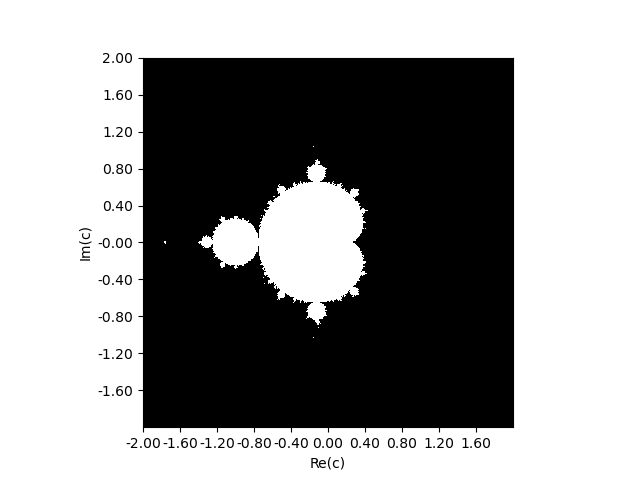
\includegraphics{ps2-4.png}
    \label{plot}%
\end{table}%

\section{Problem 5: Exercise 4.2 of Newman}

We have written the code separately in p2-5a.py, p2-5b.py, quadratic.py and test\_quadratic.py. There's two root for the function $0.001x^2 + 1000x + 0.001 = 0$. The exact number is $x_1 = -9.99989*10^{-7}$ and $x_2 = -1*10^6$. For program p2-5a.py and p2-5b.py, it requires inputing a b and c in the command line(such as writing "python3 p2-5a.py 0.001 1000 0.001")

\begin{itemize}
    \item Buy using the calculation in method A($x = \frac{-b\pm \sqrt{b^2-4ac}}{2a}$) we get $x_1 = -9.999894245993346*10^{-7}$ ,$x_2 = -9.99999999999*10^{5}$
    \item Buy using the calculation in method B($x = \frac{2c}{-b\mp \sqrt{b^2-4ac}}$) we get $x_1 = -1.000000000001*10^{-6}$ ,$x_2 = -1.0000105755125057*10^{5}$
    \item We can clearly see that the method A give more accurate result in root $x_2$ while method B give more accurate result in root $x_1$. This is because we should avoid having two large float number(which is close to each other) doing substraction against each other. In this case, when b is much larger than a and c(and is a positive number), we should avoid doing substraction such as $b - \sqrt{b^2-4ac}$. And when |b| is much larger than a and c(and b is a negative number), we should avoid doing addition such as $b + \sqrt{b^2-4ac}$.
    \item By using what has been learned, we've introduced the program C(quadratic.py) which can give more accurate result of both roots. We made it a module and can pass the test of test\_quadratic.py.
\end{itemize}













\end{document}